\documentclass{article}

\title{Dummit \& Foote Ch. 2.5: The Lattice of Subgroups of a Group}
\author{Scott Donaldson}
\date{Aug. 2023}
\usepackage{amsmath, amsthm, amsfonts, enumitem, tabu, tikz}

\tikzset{white border/.style={preaction={draw,white,line width=4pt}}}
\newcommand{\gen}[1]{$\langle#1\rangle$} % node text

\begin{document}

\maketitle

\section*{1. (8/11/23)}

Let $H$ and $K$ be subgroups of $G$. Exhibit all possible sublattices which show only $G$, 1, $H$, $K$, and their joins and intersections. What distinguishes the different drawings?

\vspace{0.5cm}

\noindent
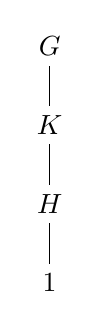
\begin{tikzpicture}
    \node at (0,0)    (I)  {$1$};
    \node at (0,1)    (H) {$H$};
    \node at (0,2)    (K) {$K$};
    \node at (0,3)    (G)  {$G$};
    
    \draw (I) -- (H);
    \draw (H) -- (K);
    \draw (K) -- (G);
\end{tikzpicture}
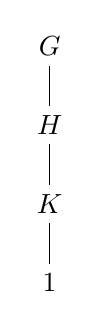
\begin{tikzpicture}
    \node at (0,0)    (I)  {$1$};
    \node at (0,1)    (K) {$K$};
    \node at (0,2)    (H) {$H$};
    \node at (0,3)    (G)  {$G$};
    
    \draw (I) -- (K);
    \draw (K) -- (H);
    \draw (H) -- (G);
\end{tikzpicture}
\begin{tikzpicture}
    \node at (0,0)    (I)  {$1$};
    \node at (1,1.5)    (K) {$K$};
    \node at (-1,1.5)    (H) {$H$};
    \node at (0,3)    (G)  {$G$};
    
    \draw (I) -- (K);
    \draw (I) -- (H);
    \draw (H) -- (G);
    \draw (K) -- (G);
\end{tikzpicture}
\begin{tikzpicture}
    \node at (0,0)    (I)  {$1$};
    \node at (0,1)    (HintK) {$H \cap K$};
    \node at (1,2)   (K) {$K$};
    \node at (-1,2)    (H) {$H$};
    \node at (0,3)    (G)  {$G$};
    
    \draw (I) -- (HintK);
    \draw (HintK) -- (H);
    \draw (HintK) -- (K);
    \draw (H) -- (G);
    \draw (K) -- (G);
\end{tikzpicture}
\begin{tikzpicture}
    \node at (0,0)    (I)  {$1$};
    \node at (1,1)   (K) {$K$};
    \node at (-1,1)    (H) {$H$};
    \node at (0,2)    (HK) {\gen{H,K}};
    \node at (0,3)    (G)  {$G$};
    
    \draw (I) -- (H);
    \draw (I) -- (K);
    \draw (H) -- (HK);
    \draw (K) -- (HK);
    \draw (HK) -- (G);
\end{tikzpicture}
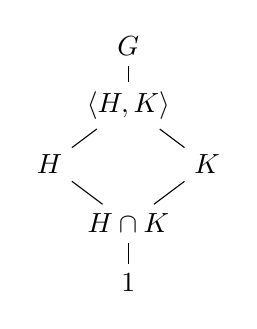
\begin{tikzpicture}
    \node at (0,0)    (I)  {$1$};
    \node at (0,0.75)    (HintK) {$H \cap K$};
    \node at (1,1.5)    (K) {$K$};
    \node at (-1,1.5)   (H) {$H$};
    \node at (0,2.25)    (HK) {\gen{H,K}};
    \node at (0,3)    (G)  {$G$};
    
    \draw (I) -- (HintK);
    \draw (HintK) -- (H);
    \draw (HintK) -- (K);
    \draw (H) -- (HK);
    \draw (K) -- (HK);
    \draw (HK) -- (G);
\end{tikzpicture}

\vspace{0.5cm}

The left two lattices show the group structure when either $H \leq K$ or $K \leq H$ (they omit any subgroups of the smaller of the two, as well as any containing subgroups between the larger and $G$).

The next lattice shows the group structure when $H$ and $K$ are not comparable, their intersection consists only of the identity, and their join is all of $G$. The final three lattices show the cases where $H \cap K$ is a subgroup not equal to the identity, where $\langle H, K \rangle$ is a subgroup not equal to $G$, and where both of these occur.

\section*{2. (8/11/23)}

In each of (a) to (d) list all subgroups of $D_{16}$ that satisfy the given condition.

\begin{enumerate}[label=(\alph*), itemsep=0em]
    \item Subgroups that are contained in $\langle sr^2, r^4 \rangle$

          $\{ 1 \}, \langle sr^6 \rangle, \langle sr^2 \rangle, \langle r^4 \rangle$, $\langle sr^2, r^4 \rangle$
    \item Subgroups that are contained in $\langle sr^7, r^4 \rangle$

        $\{ 1 \}, \langle sr^3 \rangle, \langle sr^7 \rangle, \langle r^4 \rangle$, $\langle sr^7, r^4 \rangle$
    \item Subgroups that contain $\langle r^4 \rangle$

        $\langle r^4 \rangle$, $\langle sr^2, r^4 \rangle, \langle s, r^4 \rangle, \langle r^2 \rangle, \langle sr^3, r^4 \rangle, \langle sr^5, r^4 \rangle, \langle s, r^2 \rangle, \langle r \rangle, \langle sr, r^2 \rangle, D_{16}$
    \item Subgroups that contain $\langle s \rangle$

        $\langle s \rangle$, $\langle s, r^4 \rangle, \langle s, r^2 \rangle, \langle D_{16} \rangle$
\end{enumerate}

\section*{3. (8/11/23)}

Show that the subgroup $\langle s, r^2 \rangle$ of $D_8$ is isomorphic to $V_4$.

\begin{proof}
    The subgroup $\langle s, r^2 \rangle$ of $D_8$ contains the elements $\{ 1, s, r^2, sr^2 \}$. There is no element in this group of order 4. From Ch. 1.1, Exercise 36, there is only one unique group of order 4 with no element of order 4, the Klein group $V_4$. Thus $\langle s, r^2 \rangle$ is isomorphic to $V_4$.
\end{proof}

\section*{4. (8/14/23)}

Use the given lattice to find all pairs of elements that generate $D_8$.

\begin{proof}
    Since $D_8$ is generated by $\langle s, r \rangle$, it suffices to find pairs of elements that generate $s$ and $r$. These pairs of elements are:
    \begin{itemize}[itemsep=0em]
        \item $\langle s, r \rangle$ (trivial)
        \item $\langle s, r^3 \rangle$ ($r = (r^3)^3$)
        \item $\langle s, sr \rangle$ ($r = s \cdot sr$)
        \item $\langle s, sr^3 \rangle$ ($r = s \cdot (sr^3)^3$)
        \item $\langle sr, r \rangle$ ($s = r \cdot sr$)
        \item $\langle sr, r^2 \rangle$ ($r^3 = r^2 \cdot sr, r = (r^3)^3, s = r \cdot sr$)
        \item $\langle sr, r^3 \rangle$ ($r = (r^3)^3, s = r \cdot sr$)
        \item $\langle sr^2, r \rangle$ ($s = sr^2 \cdot r^2$)
        \item $\langle sr^2, r^3 \rangle$ ($r = (r^3)^3, s = sr^2 \cdot r^2$)
        \item $\langle sr^2, sr^3 \rangle$ ($r = sr^2 \cdot sr^3, s = sr^2 \cdot r^2$)
        \item $\langle sr^3, r \rangle$ ($s = sr^3 \cdot r$)
        \item $\langle sr^3, r^3 \rangle$ ($s = r^3 \cdot sr^3, r = s \cdot sr^3$)
    \end{itemize}
\end{proof}

\section*{5. (8/14/23)}

Use the given lattice to find all elements $x \in D_{16}$ such that $D_{16} = \langle x, s \rangle$.

\begin{proof}
    The element $x \in D_{16}$ generates $D_{16}$ together with $s$ if $r$ can be expressed as a product of $s$ and $x$:
    \begin{itemize}[itemsep=0em]
        \item $x = r$ (trivial)
        \item $x = r^3$ ($r = (r^3)^3$)
        \item $x = r^5$ ($r = (r^5)^5$)
        \item $x = r^7$ ($r = (r^7)^7$)
        \item $x = sr$ ($r = s \cdot sr$)
        \item $x = sr^3$ ($r^3 = s \cdot sr^3$, $r = (r^3)^3$)
        \item $x = sr^5$ ($r^5 = s \cdot sr^5$, $r = (r^5)^5$)
        \item $x = sr^7$ ($r^7 = s \cdot sr^7$, $r = (r^7)^7$)
    \end{itemize}
\end{proof}

\section*{6. (8/14/23)}

Find the centralizers of every element in the following groups:

\begin{enumerate}[label=(\alph*), itemsep=0em]
    \item $D_8$
          \begin{itemize}[itemsep=0em]
            \item 1: $D_8$
            \item $r, r^2, r^3$: $\langle r \rangle$
            \item $s, sr^2$: $\langle s, r^2 \rangle$
            \item $sr, sr^3$: $\langle sr, r^2 \rangle$
          \end{itemize}
    \item $Q_8$
          \begin{itemize}[itemsep=0em]
            \item 1, -1: $Q_8$
            \item $i, -i$: $\langle i \rangle$
            \item $j, -j$: $\langle j \rangle$
            \item $k, -k$: $\langle k \rangle$
          \end{itemize}
    \item $S_3$
          \begin{itemize}[itemsep=0em]
            \item $(1)$: $S_3$
            \item $(1, 2)$: $\langle (1, 2) \rangle$
            \item $(1, 3)$: $\langle (1, 3) \rangle$
            \item $(2, 3)$: $\langle (2, 3) \rangle$
            \item $(1, 2, 3), (1, 3, 2)$: $\langle (1, 2, 3) \rangle$
          \end{itemize}
    \item $D_{16}$
          \begin{itemize}[itemsep=0em]
            \item 1: $D_{16}$
            \item $r, r^2, ..., r^7$: $\langle r \rangle$
            \item $s, sr^4$: $\langle s, r^4 \rangle$
            \item $sr, sr^5$: $\langle sr, r^4 \rangle$
            \item $sr^2, sr^6$: $\langle sr^2, r^4 \rangle$
            \item $sr^3, sr^7$: $\langle sr^3, r^4 \rangle$
          \end{itemize}
\end{enumerate}

\section*{7. (8/14/23)}

Find the center of $D_{16}$.

\begin{proof}
    From the preceding exercise, the only elements that are in the centralizer of every element of $D_{16}$ are $\{ 1, r^4 \} = \langle r^4 \rangle$.
\end{proof}

\section*{8. (8/14/23)}

In each of the following groups find the normalizer of each subgroup:

\begin{enumerate}[label=(\alph*), itemsep=0em]
    \item $S_3$: The subgroups (other than $(1)$ and all of $S_3$) are the three cyclic groups generated by the each of the 2-cycles, and the group consisting of $\{ (1), (1, 2, 3), (1, 3, 2) \}$. In the case of $\langle (1, 2) \rangle$, notice that:
    \begin{equation*}
        (1, 3)(1, 2)(1, 3)^{-1} = (1, 3)(1, 2)(1, 3) = (2, 3) \notin \langle (1, 2) \rangle,
    \end{equation*}
    which implies that $(1, 3) \notin N_{S_3}((1, 2))$. By extension, no 2-cycle is in the normalizer of another 2-cycle. There is no subgroup of $S_3$ that contains a 2-cycle, a 3-cycle, but does \emph{not} contain a different 2-cycle. Therefore each cyclic subgroup of $S_3$ is its own normalizer.

    Now for the subgroup $\{ (1), (1, 2, 3), (1, 3, 2) \}$, we have $(1, 2)(1, 2, 3)(1, 2) = (1, 3, 2)$, which is included in the subgroup. It follows that the normalizer of this subgroup is all of $S_3$.
    \item $Q_8$: The elements 1 and $-1$ commute with all elements of $Q_8$, so the normalizer of $\langle -1 \rangle$ is all of $Q_8$. Consider the normalizer of $\langle i \rangle$. Now $j \cdot i \cdot j^{-1} = j \cdot i \cdot -j = -k \cdot -j = i$, so $j \in N_{Q_8}(\langle i \rangle)$. Then the normalizer of $i$ contains at least 5 elements, so it must be all of $Q_8$. By extension, every subgroup of $Q_8$ is its own normalizer.
\end{enumerate}

\section*{9. (8/14/23)}

Draw the lattices of subgroups of the following groups:

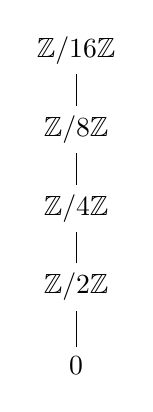
\begin{tikzpicture}
    \node at (0,0)    (1)  {$0$};
    \node at (0,1)    (2)  {$\mathbb{Z}/2\mathbb{Z}$};
    \node at (0,2)    (4)  {$\mathbb{Z}/4\mathbb{Z}$};
    \node at (0,3)    (8)  {$\mathbb{Z}/8\mathbb{Z}$};
    \node at (0,4)    (16) {$\mathbb{Z}/16\mathbb{Z}$};
    
    \draw (1) -- (2);
    \draw (2) -- (4);
    \draw (4) -- (8);
    \draw (8) -- (16);
\end{tikzpicture}\hspace{1cm}
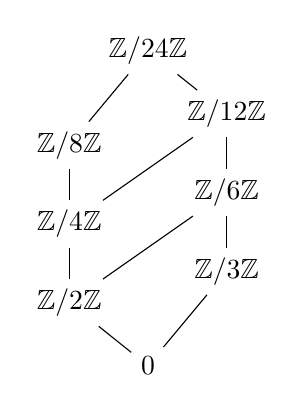
\begin{tikzpicture}
    \node at (0,0)          (1)  {$0$};
    \node at (-1,0.8)      (2)  {$\mathbb{Z}/2\mathbb{Z}$};
    \node at (1,1.2)       (3)  {$\mathbb{Z}/3\mathbb{Z}$};
    \node at (-1,1.8)      (4)  {$\mathbb{Z}/4\mathbb{Z}$};
    \node at (1,2.2)       (6)  {$\mathbb{Z}/6\mathbb{Z}$};
    \node at (-1,2.8)      (8)  {$\mathbb{Z}/8\mathbb{Z}$};
    \node at (1,3.2)       (12) {$\mathbb{Z}/12\mathbb{Z}$};
    \node at (0,4)          (24) {$\mathbb{Z}/24\mathbb{Z}$};
    
    \draw (1) -- (2);
    \draw (1) -- (3);
    \draw (2) -- (4);
    \draw (2) -- (6);
    \draw (4) -- (8);
    \draw (4) -- (12);
    \draw (8) -- (24);
    \draw (3) -- (6);
    \draw (6) -- (12);
    \draw (12) -- (24);
\end{tikzpicture}\hspace{1cm}
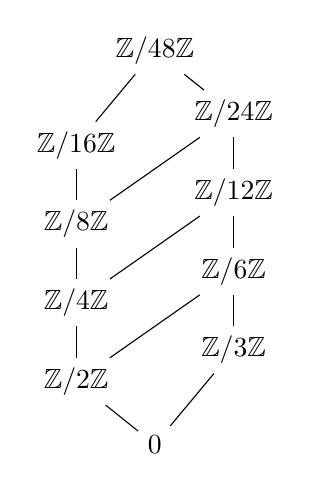
\begin{tikzpicture}
    \node at (0,0)          (1)  {$0$};
    \node at (-1,0.8)      (2)  {$\mathbb{Z}/2\mathbb{Z}$};
    \node at (1,1.2)       (3)  {$\mathbb{Z}/3\mathbb{Z}$};
    \node at (-1,1.8)      (4)  {$\mathbb{Z}/4\mathbb{Z}$};
    \node at (1,2.2)       (6)  {$\mathbb{Z}/6\mathbb{Z}$};
    \node at (-1,2.8)      (8)  {$\mathbb{Z}/8\mathbb{Z}$};
    \node at (1,3.2)       (12) {$\mathbb{Z}/12\mathbb{Z}$};
    \node at (-1,3.8)      (16)  {$\mathbb{Z}/16\mathbb{Z}$};
    \node at (1,4.2)          (24) {$\mathbb{Z}/24\mathbb{Z}$};
    \node at (0,5)          (48) {$\mathbb{Z}/48\mathbb{Z}$};
    
    \draw (1) -- (2);
    \draw (1) -- (3);
    \draw (2) -- (4);
    \draw (2) -- (6);
    \draw (4) -- (8);
    \draw (4) -- (12);
    \draw (8) -- (24);
    \draw (8) -- (16);
    \draw (3) -- (6);
    \draw (6) -- (12);
    \draw (12) -- (24);
    \draw (16) -- (48);
    \draw (24) -- (48);
\end{tikzpicture}

\section*{10. (8/15/23)}

Classify groups of order 4 by proving that if $|G| = 4$ then $G \cong Z_4$ or $G \cong V_4$.

\begin{proof}
    From Ch. 1.1, Exercise 36, if $G$ is a group with 4 elements and no element of order 4, then we must have $G = \langle a, b \mid a^2 = b^2 = 1, ab = ba \rangle \cong V_4$.

    If $G$ does have an element of order 4, then we have the cyclic group $G = \langle a \mid a^4 = 1 \rangle \cong Z_4$. All cyclic groups of equal order are isomorphic.

    Therefore a group of order 4 must be isomorphic to either the cyclic group of order 4 or the Klein 4-group.
\end{proof}

\end{document}